\chapter{Подход к решению задачи}
\label{ch:problem_solving}

В данной главе будет разобран подход к решению задачи,
которая была описана в разделе~\ref{sec:problem_formulation}.

В разделе~\ref{sec:general_approach} описана общая схема
решения поставленной в рамках настоящего исследования задачи.
Схема решения задачи состоит из двух этапов.

В разделе~\ref{sec:step1_artist_user_matrix} описаны методы,
применяющиеся на первом этапе общей схемы решания.

В разделе~\ref{sec:step2_user_feature_matrix} описаны методы,
применяющиеся на втором этапе общей схемы решения.

\section{Общая схема решения}
\label{sec:general_approach}

Предлагается решать задачу, поставленную в рамках настоящего
исследования (см. раздел~\ref{sec:problem_formulation}),
используя методики, применяемые в задачах, связанных с анализом
текста. Пользователей можно рассматривать как документы, а
названия исполнителей~--- как термины. Это даёт возможность
построить матрицу <<исполнитель-пользователь>>, по аналогии
с процедурой построения матрицы <<термин-документ>>. Таким
образом, каждый столбец данной матрицы, будет описывать
численным вектором конкретного пользователя.

Размерность матрицы <<исполнитель-пользователь>>, как
правило, оказывается очень большой, в виду того, что
общее число исполнителей велико, тогда как последовательность
исполнителей, описывающих конкретного пользователя мала
(в поставленной задаче не более 50 исполнителей для каждого
пользователя). Это не позволяет использовать вектора-столбцы
данной матрицы для описания пользователей в алгоритмах
машинного обучения ввиду проблемы переобучения и долгой
работы алгоритмов. Поэтому требуется применить техники,
позволяющие описать пользователей более компактными
численными векторами.

Таким образом схема решения состоит из двух этапов:
вычисление матрицы <<исполнитель-пользователь>>; вычисление
матрицы <<пользователь-признак>>, каждая строка которой
будет описывать пользователя через компактный численный вектор,
пригодный для использования в алгоритмах машинного обучения.
На рисунке~\ref{fig:general_approach} проиллюстрирована
общая схема предлагаемого подхода к решению задачи. Как видно
из рисунка, каждый из двух этапов предлагается
выполнять одним из двух способов.

\begin{figure}[!h]
\caption{Общая схема решения задачи профилирования пользователей
         по их музыкальным предпочтениям}
\label{fig:general_approach}
\centering
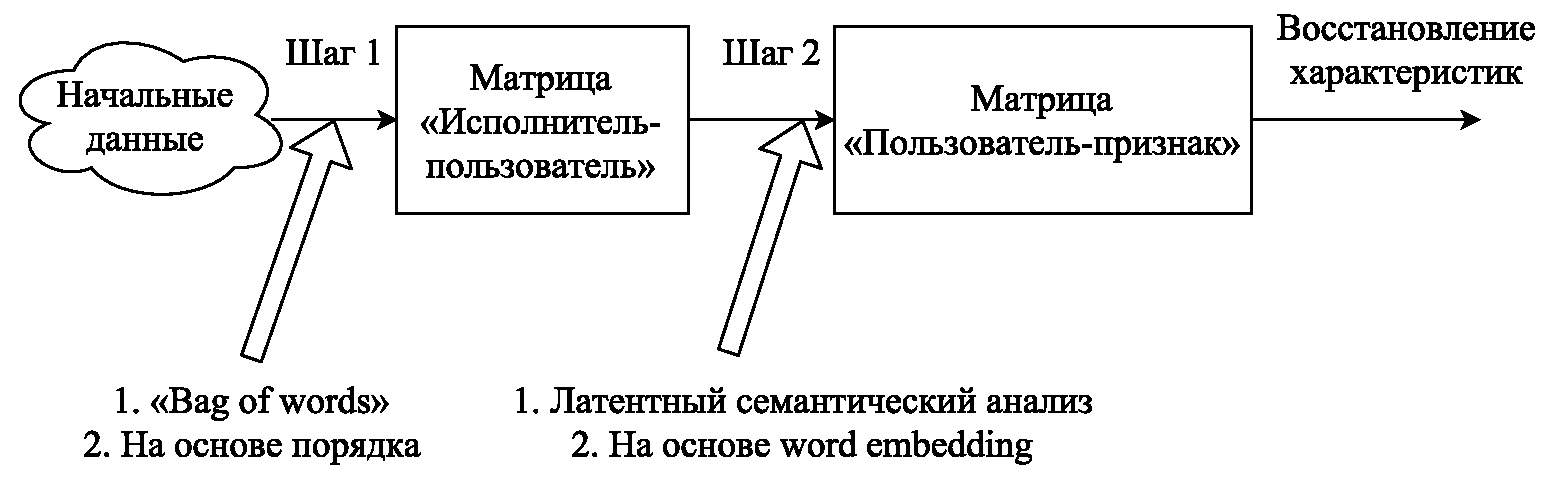
\includegraphics[width=\textwidth]{figs/general-approach.pdf}
\end{figure}

В последующих разделах будут рассмотрены все варианты,
позволяющие выполнить первый и второй шаг, предлагаемого
подхода к решению задачи.

\section{Построение матрицы <<исполнитель-пользователь>>}
\label{sec:step1_artist_user_matrix}

В настоящем разделе описаны подходы, позволяющие выполнить
первый шаг описанного подхода к решению задачи профилирования
пользователей на основе анализа их музыкальных предпочтений.

\subsection{Подход <<bag of words>>}

Вычисление матрицы <<исполнитель-пользователь>> может быть
реализовано на основе предположения <<bag of words>>, то есть
без учёта порядка следования исполнителей, описывающих пользователей.

Предлагается, используя обобщённую формулу TF-IDF 
(см. формулу~\ref{eq:general_tfidf}) или формулу log-entropy
(см. формулу~\ref{eq:log_entropy}), вычислить данную матрицу.

Подробное рассмотрение процедуры вычисления матрицы <<термин-документ>>
(в данном случае <<исполнитель-пользователь>>) на основе
предположения <<bag of words>> было описано в 
разделе~\ref{sec:term_document_matrix}.

\subsection{Подход на основе порядка следования исполнителей}

Вычисление матрицы <<исполнитель-пользователь>> может быть
также реализовано с учётом порядка следования исполнителей,
описывающих пользователей. 

Исполнители, описывающие конкретного пользователя, следуют
в определённом порядке~--- по убыванию числа прослушиваний
пользователем музыкальных композиций (подробнее было описано
в разделе~\ref{sec:problem_formulation}). Таким образом,
имеет место гипотеза о том, что чем выше находится исполнитель
в списке у пользователя, тем лучше данный исполнитель
<<описывает>> пользователя. Опираясь на эту гипотезу, можно
предложить способ вычисления элементов матрицы
<<исполнитель-пользователь>>. 

Пусть имеется множество пользователей:
\[
    \mathcal{D} = \{\mathcal{D}_1, \mathcal{D}_2,..., \mathcal{D}_n\},
\]
а также множество исполнителей:
\[
    T = \{t_1, t_2,..., t_m\}.
\] 
Введём вспомогательные множества:
\[
    A_{ij} = \{k \colon a_k \in D_j \land a_k = t_i\}.
\]
Таким образом множество $A_{ij}$ содержит в себе номера
позиций, на которых находится исполнитель $i$ у
пользователя $j$. Тогда, основываясь на упомянутой гипотезе,
можно предложить следующую формулу для вычисление коэффициентов
матрицы <<исполнитель-пользователь>> $D$:
\begin{equation}\label{eq:order_dij}
    d_{ij} = \begin{cases}
          0,& A_{ij} = \varnothing,\\
          \sum\limits_{a \in A_{ij}}{f(a)},& A_{ij} \ne \varnothing,
      \end{cases}
\end{equation}
где $f$~--- произвольная неотрицательная невозрастающая функция,
определённая на промежутке $\left[1, 50\right]$. Такая область
определения функции $f$ обусловлена тем фактом, что каждый
пользователь описан не более, чем 50 исполнителями.

Описанная выше формула <<наделяет>> исполнителя большим
весом, если он находится высоко в списке пользователя, и
небольшим~--- иначе. При этом, так как исполнители,
описывающие конкретного пользователя, могут повторяться,
то такая формула даёт возможность учитывать как число
встреч исполнителей, так и позиции, на которых они находятся.

\section{Построение матрицы <<пользователь-признак>>}
\label{sec:step2_user_feature_matrix}

В настоящем разделе описаны подходы, позволяющие выполнить
второй шаг описанного подхода к решению задачи профилирования
пользователей на основе анализа их музыкальных предпочтений.

\subsection{Подход на основе латентного семантического анализа}

Техника латентного семантического анализа (по крайней мере
вероятностные подходы) зиждется на гипотезе о существовании
латентных тематик, к которым можно отнести термины и документы.

В случае решаемой задачи в рамках настоящего исследования,
можно предположить, что каждого исполнителя возможно отнести
к нескольким музыкальным жанрам, а каждый пользователь может быть
описан жанрами, которые он предпочитает.

Таким образом, пусть $D$~--- матрица <<исполнитель-пользователь>>,
тогда, решая задачу латентного семантического анализа, можно
получить следующее:
\[
    D = U \cdot V^T,
\]
где матрица $U$ описывает исполнителя через жанры, а матрица
$V$~--- пользователей. Выбрав размерность столбцов этих
матриц сильно меньше общего числа строк матрицы $D$ (числа
исполнителей), появляется возможность использовать матрицу $V$
(матрица <<пользователь-признак>>) в алгоритмах машинного обучения.  
В случае подходов, не основанных на вероятностной модели порождения
данных, латентного семантического анализа, вряд ли можно говорить о
<<скрытых>> музыкальных жанрах, но, тем не менее, снизить размерность
матрицы $D$ также возможно.

Подробно техника латентного семантического анализа была описана
ранее в разделе~\ref{sec:latent_semantic_analysis}.

\subsection{Подход на основе векторного представления слов}

Векторное представление слов (или word embedding) позволяет
преобразовать словарь терминов в векторы одинаковой размерности
(см. раздел~\ref{sec:word_embedding}). 

Пусть имеется матрица <<исполнитель-пользователь>>
$D \in \mathbb{R}^{m \times n}$, вычисленная произвольным
образом. Пусть также имеется множество векторов,
описывающих исполнителей, вычисленных при помощи техники
word embedding: 
\[
    \mathcal{W} = \{\bm{w}_1, \bm{w}_2,..., \bm{w}_m\},\quad
    \forall i \in [1, m] \colon \bm{w}_i \in \mathbb{R}^k,
\]
где $k$~--- размерность векторов, описывающих исполнителей.
Из векторов, полученных при помощи word embedding, построим
матрицу $W \in \mathbb{R}^{m \times k}$. Тогда вычисление матрицы
<<пользователь-признак>> может быть выполнено следующим образом:
\[
    M = D^T \cdot W,\quad M \in \mathbb{R}^{n \times k}.
\]
Таким образом, выбрав значение $k$ много меньше значения $m$,
получаем матрицу $M$, каждая строка которой описывает
пользователя компактным вектором.

Для лучшей ясности семантики матрицы $M$, можно описать
процесс её построения несколько иначе. Строка $\bm{m}_i$ матрицы 
<<пользователь-признак>> $M$ вычисляется следующим образом:
\[
    \bm{m}_j = \sum_{i=1}^{m} d_{ij} \cdot \bm{w}_i.
\]

Предположим матрица <<исполнитель-пользователь>> построена 
таким образом, что значения её элементов $d_{ij}$ равны нулю,
если исполнитель $i$ не встречается у пользователя $j$, и равно
положительному значению иначе. Тогда разумно предположить, что
линейная комбинация векторов, описывающих исполнителей, 
в какой-то мере описывает пользователя исполнителями, которых
он предпочитает прослушивать.

\chapterconclusion

В данной главе был рассмотрен подход к решению задачи
определения характеристик пользователей на основе анализа
их музыкальных интересов, предлагаемый в рамках настоящего
исследования. 

Была рассмотрена общая схема решения поставленной задачи,
которая состоит из двух этапов. При этом каждый этап, может
быть выполнен двумя способами.

Было описано два подхода к выполнению первого этапа схемы
решения задачи: стандартный подход на основе подхода
<<bag of words>>, а также подход на основе порядка, применимый
к данной конкретной задаче.

Было описано два подхода к выполнению второго этапа схемы
решения задачи: стандартный подход на основе латентного
семантического анализа, а также подход на основе техники
word embedding.
